\chapter{Construction du corpus AlloSat}
\label{chapitre4}
"Vos clients les plus mécontents sont votre meilleure source d’apprentissage" (Bill Gates)

\section{Motivation}
L'un des objectifs de cette thèse est de comprendre et de reconnaître l'état émotionnel de clients étant en relation téléphonique avec des agents de centre d'appels. L'objectif de ces conversations sont en général soit d'acheter un produit (service d'abonnement, service d'achat), soit de régler un problème (plainte, service après vente, service de réclamation), soit de demander des informations diverses sur une entreprise ou leur produit. Selon l'exigence industrielle, deux émotions sont primordiales dans la relation clientèle : la satisfaction, facteur de fidélité et de diffusion de la marque ainsi que la frustration, facteur d'attrition du client et de "mauvaise publicité". Ces deux émotions, comme nous avons pu le voir dans le chapitre~\ref{chapitre1}, peuvent s'inscrire dans différentes théories discrètes ou continues.
Nous avons choisi de les inscrire dans un espace continu, en créant la dimension de satisfaction comme explicité dans la figure~\ref{fig:satisfactionAxis}. En effet, outre l'émotion brute, la variation de son intensité et de sa durée sont des indicateurs cruciaux pour améliorer l'expérience du client.

\begin{figure}[h]
  \centering
  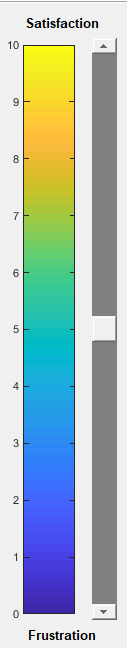
\includegraphics[width=\textwidth]{./Chapitre4/figures/satisfactionAxis.png}
  \caption{L'axe de satisfaction va de la frustration à la satisfaction, en passant par le neutre. C'est donc sur cet axe que l'annotation a été effectuée.}
  \label{fig:satisfactionAxis}
\end{figure}


Pour étudier ces émotions, nous avons besoin de données et donc d'un corpus.
Lorsque nous avons recherché un corpus, que vous pouvez retrouver au chapitre~\ref{chapitre3}, adapté à notre problématique, nous nous sommes rendu compte qu'aucun ne correspondait parfaitement à notre demande.
En effet, il existe peu de corpus comportant des conversations réelles issues de centre d'appel qui soit disponible. Nous avons donc fait le choix de créer un corpus, que nous avons rendu accessible, afin d'étudier la dimension de satisfaction dans des conversations de centre d'appels.


\section{Recueil des données}
Grâce à l'entreprise Allo-Média, nous avons pu recueillir des données provenant de différents centre d'appels français, sous forme de conversations audio entre des appelants (les clients) et des agents.
Pour ce faire, nous avons récupéré une trentaine de conversations par domaine d'activité des entreprises : de l'assurance, de la distribution d'énergie, des agences de voyages, des agences immobilières, qui ont eu lieu entre juillet 2017 et novembre 2018. Ces conversations étant séparées dans l'enregistrement entre le canal du client et le canal de l'agent, nous n'avons pas de chevauchement de signal entre les locuteurs. De plus, pour des contraintes éthiques et commerciales, la partie concernant l'agent ne peut être diffusée et a donc été supprimé des données collectées, en effet Allo-Media ne s'inscrit pas dans une logique de contrôle et de notation des agents. La partie du client quant à elle, est principalement constitué d'un locuteur unique qui ne sera pas retrouvé dans d'autres conversations. Toutefois, il existe également des conversations ou il peut y avoir plusieurs locuteurs du client, comme par exemple quand une personne passe le téléphone à un autre membre de sa famille. Tous ces audios sont issus du canal téléphonique, ce qui explique qu'il soit échantillonné en 8kHz.
Face à cette masse de données, et conscient que nous ne pourrions pas tout annoter, nous avons du mettre en place un processus pour sélectionner les données à ajouter au corpus.

\subsection{Sélection des données}
Il est communément admis que toutes les conversations traitées en centre d'appels ne se sont pas marquées par la satisfaction ou la frustration. En effet, lors d'un appel pour une précision sur la livraison d'un produit ou sur le suivi d'un abonnement par exemple, il est rare de voir des émotions exprimées. Selon truc et machin, à peine 20\% de la parole contient des aspects émotionnels.
Comme nous l'avons vu précédemment dans le chapitre~\ref{chapitre1}, la frustration peut se reconnaître par une modification du timbre, une parole plus rapide et des disfluences plus importantes. On peut également ajouter l'augmentation de la présence du para-linguistique avec des soupirs, des bruits de langues ou des rires nerveux. On a également remarqué que le discours se teinte de mots à polarité négative et présente des répétitions. Dans certains cas, on peut observer une augmentation des négations.

Fort de ces observations, afin de réduire le coût d'annotation, nous avons donc choisi de sélectionner des conversations où la présence de la satisfaction ou de la frustration peut être détectée par l'humain. Pour ce faire, nous avons mis en place plusieurs critères :
\begin{itemize}
  \item La durée de la conversation : celle-ci doit être d'au moins 30 secondes, pour avoir le temps d'exprimer une émotion. Comme la frustration et la satisfaction semble être induite par une interaction avec l'agent, nous ne conservons que les conversations composées d'au moins trois tours de parole, soit trois prises de parole de la part du client et du conseiller,
  \item La variation de la fréquence fondamentale dans l'ensemble de la conversation doit être la plus grande possible. En effet, comme nous l'avons vu précédemment, la variation de la fréquence fondamentale est une indication permettant de caractériser la prosodie de la parole. Plus elle est grande, plus la personne va utiliser une grande amplitude de timbre, qui peut être un indicateur d'émotion. Le timbre d'une personne satisfaite ou sans émotion est différente du timbre d'une personne frustrée. Afin de calculer cette fréquence fondamentale, nous avons utilisé l'algorithme YAPPT~\cite{Zahorian2008} qui permet de palier au contexte téléphonique. En effet, le signal téléphonique étant souvent de mauvaise qualité, la fréquence fondamentale peut être absente. Cet algorithme cherche donc à restaurer la fréquence fondamentale des signaux dégradés.
  \item La conversation doit être polarisée : pour ce faire, nous avons calculé un score de polarité en partant des transcription de la partie du client. En utilisant le dictionnaire French Affective Norms (FAN)~\cite{Monnier2014} qui propose un score de valence (entre 0 et 10) pour plus de 1000 mots, annoté par plus de 400 français et françaises, nous avons calculé un score de valence correspondant à la moyenne des scores de chaque mot polarisé. Les autres mots sont pris en compte avec le score de 5, considéré comme le neutre. Ce score de valence de la conversation varie donc entre 0 et 10, 0 étant le plus négatif et 10 le plus positif.
\end{itemize}
Ces critères ont permis d'isoler 180 conversations qui présentaient des caractéristiques intéressantes. Ces dernières ont été écoutées afin de garder les conversations où la manifestation de la dimension de satisfaction était la plus flagrante. Par ce procédé, nous avons conservé 253 conversations.
Afin de mieux respecter la répartition des états émotionnels dans un contexte de centre d'appels, nous avons également sélectionné au hasard 50 conversations qui n'étaient pas retenus par le filtre mis en place.
Une fois cette sélection effectuée, nous avons du traiter les données pour qu'elles puissent être annotées par la suite.

\subsection{Pre-traitement des données}

\subsubsection{Écourter les silences}
Comme les deux canaux (client et agent) sont séparés en amont, il nous a suffit de conserver uniquement les documents provenant du canal client, afin de ne pas traiter la parole de l'agent.
L'absence de la réponse du conseiller ajoute de long moment de silence dans le signal audio. Afin de réduire l'effort d'annotation, nous avons décidé de réduire les silences de plus de deux secondes. Cette réduction suit le protocole suivant :
\begin{itemize}
  \item On détecte les silences automatiquement en utilisant l'outil ffmepg. On liste les silences qui sont présentés dans le document.
  \item On découpe le signal audio dès lors que l'on trouve un silence d'une durée supérieure à deux secondes.
  \item On réassemble les fragments du signal audio, en intercalant un signal audio de bruit blanc d'une durée exacte de deux secondes.
\end{itemize}

Ce traitement nous permet de passer d'un corpus de X heures majoritairement composé de silence à un corpus de 37h où les silences sont plus contrôles. Nous avons donc une répartition des durées de conversation plus homogènes, qui est décrites dans la figure~\ref{fig:repart}. Les conversations ont une durée variant de 32 secondes à 41 minutes, avec une moyenne d'environ 7 minutes.
\begin{figure}[h]
  \centering
  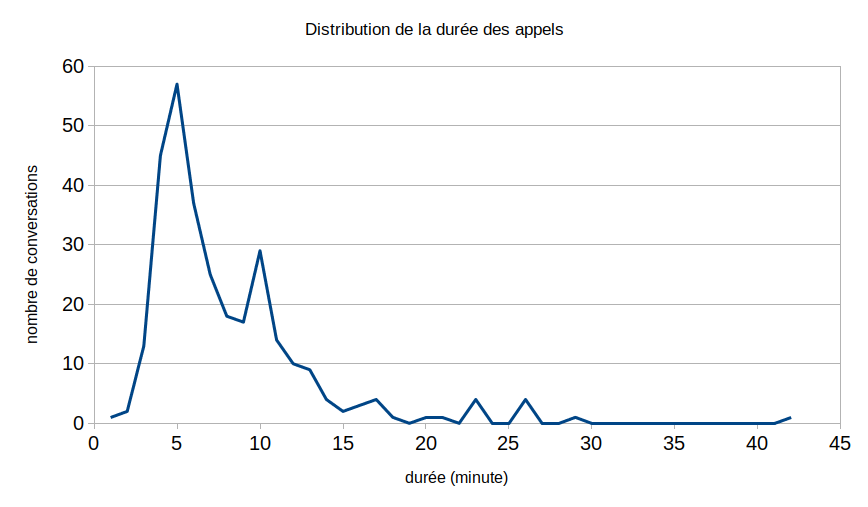
\includegraphics[width=15cm]{./Chapitre4/figures/repart.png}
  \caption{La répartition des conversations en fonction de leur durée. En bleu, nous avons les anciennes durées, en orange les nouvelles. Environ $76,6\%$ des conversations duraient moins de 15 minutes (soit 900 secondes). Après réduction des silences, ce nombre augmente à environ $93,7\%$.}
  \label{fig:repart}
\end{figure}


\subsubsection{Anonymiser les données personnelles}
Afin de respecter la vie privée des clients, la France et d'autres pays européens ont mis en place une réglementation du stockage des données personnelles de tout individu. Le règlement général sur la protection des données (RGPD) établit des règles relatives à la protection des utilisateurs vis à vis du traitement de leur données personnelles, pour s'assurer que les utilisateurs conservent leurs libertés et leurs droits fondamentaux. Cette réglementation, contrôlée par la Commission Nationale de l'Informatique et des Libertés (CNIL) a été renforcée en 2018, afin de mieux protéger les données personnelles des individus.
Nous avons donc obfusqués les données personnelles pour être en adéquation avec les réglementations de la RGPD. Les données personnelles anonymisées sont présentées dans le tableau~\ref{tab:donneesPerso}. À ces dernières s'ajoutent les données permettant d'identifier les entreprises suscitées : les marques et les produits proposées par ces entreprises. Ainsi, les conversations finales permettent de reconnaître le domaine d'activité de l'entreprise mais pas son identité.
Pour procéder à cette obfuscation, une première passe d'un obfuscateur automatique, détenu par la société Allo-Média, a été passée sur les fichiers audio. En reconnaissant les entités nommées sur les transcriptions de ces audios, ce parseur substitue le segment audio correspondant au timecode de l’entité nommée détectée par un signal audio préenregistré qui se compose d'un ait de percussion de type jazzy.
Une deuxième passe, humaine cette fois ci, permet de garantir l'obfuscation de toutes les données personnelles. En utilisant l'outil Transcriber, chaque conversation a été écouté et lu en parallèle, permettant d'identifier et de segmenter les données personnelles encore présentes. C'est lors de cette deuxième phase que les données permettant d'identifier les entreprises ont été isolées. Nous avons également choisi de supprimer tous les numéros permettant d'identifier un contrat ou une date significative.
Les segments identifiés sont alors substitués par le même signal audio jazzy. Une fois ce traitement effectués, nous avons pu passer à l'annotation.

\section{Mise en place de l'annotation}

\subsection{Les deux annotations}
Comme nous l'avons dit précédemment, nous souhaiter analyser l'axe de satisfaction de manière continue. Pour cela, nous avons mis en place un axe dont les extremum sont la frustration (0) et la satisfaction (10) qui passe par un état neutre (5) situé à mi-chemin entre ces deux émotions comme montré dans la figure~\ref{fig:satisfactionAxis}. La valeur de satisfaction est extraite toutes les 250ms, ce qui nous permet d'avoir 4 valeurs par seconde. Nous avons fait ce choix parce que, contrairement aux mots qui seront analysés dans des fenêtres de 30ms pour la reconnaissance automatique de la parole, les émotions s'expriment sur une période de temps plus longue, généralement de l'ordre de la minute~\cite{Schuller2010}. Cette annotation étant influencé par l'affect des annotateurs, nous avons cherché des moyens de valider cette annotation, que ce soit entre différents annotateurs ou même intrinsèque à l'annotateur.

Pour ce faire, nous avons décidé de mettre en place, en plus de l'annotation continue, une annotation discrète de la dimension de satisfaction. Cette annotation discrète est effectuée au niveau de la conversation. Elle relève la catégorie émotionnelle du début et de fin de conversation, comprise entre très frustré, frustré, neutre, satisfait, très satisfait. En plus, une caractérisation de l'évolution de l'émotion est annotée selon les catégories suivante : montante, descendante, stagnante, varie, varie fortement. Pour mieux comprendre ces catégories, elles sont présentées dans la figure~\ref{fig:variation}.
\begin{figure}
  \centering
  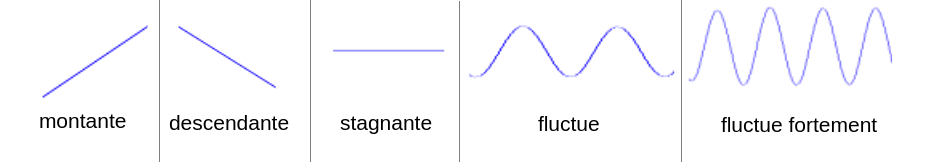
\includegraphics[width=14cm]{./Chapitre4/figures/variation.png}
  \caption{Schéma des variations qui ont été données aux annotateurs afin de mieux comprendre la catégorie évolution}
  \label{fig:variation}
\end{figure}

Dans un objectif de diffusion du corpus, et donc de pouvoir le comprendre aux corpus existant, nous avons également mis en place une annotation de la valence sur le même principe que l'annotation discrète de la dimension de la satisfaction. Elle relève la valence du début et de fin de conversation, comprise entre très négative, négative, neutre, positive, très positive. On y ajoute la même caractérisation de l'évolution de la valence.
La différence entre la dimension de satisfaction et la valence a fait l'objet de plusieurs séances d'explication, afin que ces deux notions ne sont pas confondues par les annotateurs.

\subsection{Contexte donné aux annotateurs}
Afin d'aider les annotateurs et de guider au mieux l'annotation, un guide d'annotation a été mis à leur disposition(disponible dans l'annexe~\ref{ap:guidelines}). Ce dernier explique le contexte de l'étude et les consignes à respecter. Comme l'émotion possède une part non négligeable de subjectivité, il fallait que les consignes soient les plus objectives possibles.
Pour expliquer la notion de valence, nous avons utilisé le Self-Assessment Manikin (SAM)~\cite{SAM} qui donne une description visuelle de la valence, que l'on retrouve sur la figure~\ref{fig:SAM}.
\begin{figure}
  \centering
  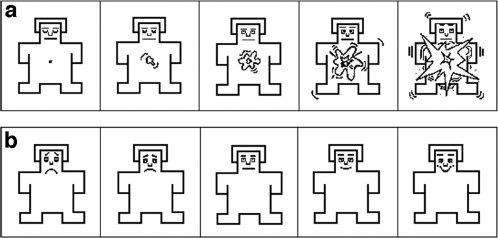
\includegraphics[width=12cm]{./Chapitre4/figures/sam.jpeg}
  \caption{Le Self Assessment Manikin (SAM). La ligne a correspond à l'activation, la ligne b correspond à la valence.}
  \label{fig:SAM}
\end{figure}

Nous nous concentrons sur deux notions :
\begin{itemize}
  \item L'évolution d'une émotion : tous les appels commencent au 'neutre' et évoluent en fonction du temps entre frustration et satisfaction. Cette annotation est continue.
  \item Une évaluation de l'émotion à posteriori : une fois l'appel terminé, nous voulons avoir un retour sur l'évolution de l'émotion. Pour cela nous voulons savoir comment était l'appelant au début de la conversation, comment il était à la fin et comment était l'évolution. Cette annotation est donc discrète.
\end{itemize}

Pour palier à l'aspect subjectif, ils ont été informés que tous les annotateurs annotent les mêmes conversations. Comme l'empathie peut avoir un grand impact sur l'annotation des émotions, nous avons demandé aux annotateurs d'être le plus objectif dans leur annotation et de ne pas prendre partie pour le client.

\subsection{Logiciel utilisé}

Pour réaliser l'annotation continue, CARMA (Continuous Affect Rating And Media Annotation)~\cite{CARMA} est le logiciel d'annotation que nous avons retenu pour cette tâche. Inspiré de FeelTrace~\cite{FeelTrace}, l'outil le plus utilisé pour faire des annotations continues d'émotions, il permet d'annoter de façon continue l'émotion selon une dimension définie en amont. Nous avons choisi CARMA puisque contrairement à FeelTrace, un simple clavier et une souris permettent de mettre en pratique l'annotation. FeelTrace quant à lui, nécessite l'utilisation d'un joystick, qu'il faut se procurer et configurer. De plus, l’outil est optimisé pour annoter deux dimensions à la fois, la valence et l'activation, afin de placer l'annotation dans un contexte bi-dimensionnel qui ne correspond pas avec notre définition de l'axe de satisfaction.

Pour l'annotation discrète, les annotateurs ont rempli un modèle préconstruit vide d'Excel que nous détaillerons par la suite.

\subsection{Consignes}

L'annotation doit être réalisée sur la dimension de satisfaction de façon continue selon les consignes suivantes :
\begin{itemize}
  \item La barre d'annotation va de 0 (Frustration) à 10 (Satisfaction) et est graduée par palier de 1. Le 5 correspond à l'état neutre et à l'état de départ de l'annotation.
  \item Le curseur d'annotation peut être contrôlé par la souris ou par les flèches du clavier. Les pas du clavier sont de 0.1 tandis que la souris peut avoir une granularité plus fine.
  \item Si aucun état émotionnel n'est constaté, ou qu'il ne varie pas, alors l'annotateur ne doit pas toucher à l'annotation. Cela est valable également lors des silences. Les annotateurs ont été notifiés de la présence de conversation où aucun état émotionnel n'a été constaté.
  \item Un document ne doit être annoté qu'une seule fois par la même personne, sans possibilité de revenir en arrière. Il n'est pas non plus possible d'avancer la conversation, l'annotation doit être faite en temps réel de l'écoute de la conversation.
  \item Un document doit être annoté en une seule fois. On ne doit pas revenir à l'annotation d'un fichier après une longue pause (plusieurs heures ou un jour). Cela évite à l'annotateur de ne plus être dans le contexte émotionnel de la conversation.
\end{itemize}

Ces consignes ont pour but d'aider l'annotateur a faire l'annotation la plus objective possible. En plus de ces consignes, la structuration des documents a été expliqué. Les bruit blanc indique qu'un silence de plus de 2 secondes s'est produit. Il a été retiré du document pour fluidifier l'écoute et l'annotation du document. Ce son est à titre informatif pour aider dans l'annotation. Tandis que  les bruits jazzy sont utilisés pour l'anonymisation des conversations. Il remplace les parties de conversation où des données personnelles tel que le nom des personnes ou permettant l'identification de l'entreprise sont prononcées.

Pour leur permettre d'avoir une meilleure compréhension de la satisfaction et de la frustration que nous voulons retrouver, nous avons fourni deux conversations en temps que borne de satisfaction et borne de frustration, afin de calibrer tous les annotateurs, qu'il puisse appréhender l'amplitude potentielle de la dimension de satisfaction.

Pour ce qui est des dimensions discrètes, les consignes stipulent qu'elles doivent être annotées tout de suite après l'écoute de la conversation, afin que les états émotionnels ne soient pas oubliés ou pollués par l'écoute d'autres conversations.
Six catégories sont donc à remplir à la fin de chaque annotation: la dimension de satisfaction de début et de fin de conversation avec la force de l'évolution temporaire; les mêmes informations ont été demandées pour la dimension de la valence.

\section{Analyse de la qualité d'AlloSat}
AlloSat est composé de 303 conversations, d'une durée totale de 37 heures 23 minutes et 27 secondes, et le discours est prononcé par 308 locuteurs distincts dont 191 femmes et 117 hommes.
Ces conversations ont été annotées par trois annotateurs, 2 femmes et 1 homme, formés à la transcription d'appels et à l'annotation en catégorie discrètes de concepts sémantiques.
Une répartition en trois ensembles a été définies. L'ensemble d’entraînement (train) est composé de 201 conversations, le développement de 42 conversations et le test de 60 conversations. De plus amples détails sont disponibles dans le tableau~\ref{tab:repartitionEnSets}.
\begin{table}[]
\begin{tabular}{|l|l|l|l|}
\hline
      & Nombre de conversations & Durée    & Durée de parole \\ \hline
TRAIN & 201                     & 25h26m35 & 15h48m50        \\ \hline
DEV   & 42                      & 05h55m46 & 03h22m14        \\ \hline
TEST  & 60                      & 05h58m41 & 03h28m57        \\ \hline
\end{tabular}
\caption{Découpage du corpus en ensemble de train, développement et test. Les durées sont données en heures, minutes, secondes.}
\label{tab:repartitionEnSets}
\end{table}


Afin de statuer sur la qualité du corpus, nous avons étudiés l'annotation de ces trois annotateurs : nous avons mis en place des mesures d'accord intra-annotateurs, permettant de mesurer la pertinence d'une annotation vis à vis des autres annotations du même annotateur et d'accord inter-annotateurs, permettant de mesure la pertinence de l'annotation d'un document par rapport à une autre annotation du même document.
Le tableau~\ref{tab:statistiqueAnnotation} regroupe l'usage des annotations discrètes de corpus. Nous pouvons observer une sur-représentation de l'état neutre, qui est en adéquation avec la part émotive que l'on s'attendait à trouver dans la parole. Comme nous le pensions, la plupart des conversations ont été perçues avec une frustration croissante, probablement parce que le conseiller n’est pas en mesure de donner une réponse suffisamment satisfaisante à l’interlocuteur.

\subsection{Accord intra-annotateur}
Pour mesurer l'accord intra-annotateur, nous avons choisi de comparer les annotations continues aux annotations discrètes. Comme nous pouvons le voir sur la table~\ref{tab:statistiqueAnnotation}, peu de conversations ont été annotées en très satisfait. Nous avons donc choisi de regrouper les catégories très satisfaites et satisfaites. Afin de rester symétrique dans nos annotations, nous avons également regroupé les catégories très frustrées et frustrées. Les annotations discrètes sont ensuite fusionnées par vote majoritaire. Nous avons eu un cas de désaccord total, dans ce cas nous avons choisi de prendre en compte l'annotation de l'annotateur ayant le plus haut coefficient de corrélation.
Cet accord est mesuré entre les annotations continues et discrètes d'une même conversation par un même annotateur. Les annotations continues ont été normalisées en suivant la méthode de la normalisation min/max, remettant les annotations dans un espace allant de 0 à 1.
Nous avons discrétisés ces valeurs, appelée Sn, pour se synchroniser avec l'annotation discrète. Pour ce faire, nous avons définis deux seuils permettant de déterminer si une valeur continue correspond à un état de frustration (Sn<0.45), à un état neutre (0.45 < Sn < 0.55) ou à un état de satisfaction (Sn > 0.55). Ces seuils ont été définis empiriquement par observation de l'annotation des conversations neutres contenues dans le corpus.
Ensuite nous avons définis les notions de début et fin de conversation dans le contexte de l'annotation continue. Nous avons déterminé qu'il était chacun constitué de 10\% de la durée totale de la conversation. Le début correspond au segment commençant à 0 et finissant à 0.1*durée totale de la conversation et la fin correspond au segment commençant par la durée totale - 0.1*durée de la conversation, jusqu'à la fin de la conversation.
Nous avons alors fait la moyenne des annotations qui représentent le début de la conversation et nous appliquons le seuillage pour déterminer quelle étiquette caractérise cette intervalle de temps. Nous faisons exactement la même chose avec les annotations de fin de conversation. Ainsi pour chaque conversation, nous avons l'annotation discrète effectuée par l'annotateur et une autre annotation discrète correspondant à la discrétisation de son annotation continue.
La différence entre l'annotation discrétisée du début et de la fin devrait être en adéquation avec l'évolution annotée.
Ce processus nous permet de calculer un kappa par annotateur.
Le kappa (k) est une mesure permettant de quantifier l'accord entre deux observations. Elle mesure le degré de concordance entre deux observation selon l'équation suivante\ref{eq:kappa}:
\begin{equation}
    \kappa = \dfrac{P_0 - P_e}{1 - P_e}
    \label{eq:kappa}
\end{equation}
$P_0$ correspond à l'accord relatif entre annotations et $P_e$ représente la probabilité d'un accord aléatoire. Comme nous avons un cas de sur-représentation d'une classe, ici le neutre, nous avons fixé $P_e$ à 1/3~\cite{Callejas2008}.
Le kappa est compris entre 0 et 1. Plus le kappa est proche de 1, plus l'accord entre les deux observations est forte. En revanche, plus le kappa se rapproche de 0 et moins on a d'accord entre les observations.

\begin{table}[th]
  \centering
  \begin{tabular}{|p{2cm}| l l | l l|}
    \hline
        &\multicolumn{2}{c}{\textbf{Nombre de désaccord}} & \multicolumn{2}{c}{\textbf{kappa}} \\
              &début  &fin    &début      &fin  \\
    \hline
    a1        &4      &31     &0.98       &0.84	\\
    a2        &23     &55     &0.88       &0.72 \\
    a3        &13     &50     &0.93       &0.75	\\
    \hline
    Moyenne  &13.33 &45.33 &0.93   &0.77 \\
    \hline
  \end{tabular}
\caption{Nombre de désaccord et kappa pour définir l'accord intra-annotateur pour chacun des trois annotateurs ainsi que la moyenne. $a_i$ represente l'annotateur $i$.}
\label{tab:accordIntraAnnot}
\end{table}

Les résultats de ces calculs sont disponibles dans le tableau~\ref{tab:accordIntraAnnot}. Nous pouvons observer une forte concordance entre les annotations discrètes et les annotations continues discrétisées dans les début de conversation avec un kappa moyen de 0.93. Si on se penche sur le nombre de cas où l'annotation discrète et différente de l'annotation continue discrétisée, on voit que le premier annotateurs et a environ 1\% de différence et qu'au maximum, l'annotateur 2 a une différence de moins de 8\%.
Pour les fins de conversation, on observe de moins bon score, avec un kappa moyen de 0.77 mais qui reste suffisant pour exprimer une cohérence des annotations. En regardant le nombre d'annotations différentes, on observe de nouveau que l'annotateur 1 a le moins de différences avec moins de 10\%, tandis que l'annotateur 2 monte à presque 17\% de différence.
Nous avons conclu que, même si l'accord intra-annotateur n'est pas parfait, il est suffisant pour certifier de la cohérence des annotations produites par un même annotateur : les annotations discrètes et continues sont cohérentes l'une envers l'autre.

\subsection{Accord inter-annotateur}
Afin d’évaluer l’accord inter-annotateur sur les annotations continues, nous avons utilisé le coefficient de corrélation linéaire. Ce coefficient est calculé au niveau de la conversation sur la satisfaction normalisée par rapport à l’ensemble des conversations entre les paires d’annotateurs comme défini dans la section précédente.

Le coefficient de corrélation linéaire donne une mesure de l'intensité et du sens de la relation linéaire entre deux variables, ici les deux annotations de deux annotateurs. Son calcul est définit par l'équation suivante~\ref{eq:coeffCorr}:
\begin{equation}
  \r = \dfrac{Cov(x,y)}{\sigma_x \sigma_y}
  \label{eq:coeffCorr}
\end{equation}
où $Cov(x,y)$ désigne la covariance entre les variables x et y, ici l'ensemble des annotations de deux annotateurs et $\sigma_x$ $\sigma_y$ désignent leur écart type.
Il est compris entre -1 et 1. Plus le coefficient est proche de 1, plus la relation linéaire positive entre les variables est forte. Plus le coefficient est proche de -1, plus la relation linéaire négative entre les variables est forte. Si le coefficient est proche de 0, on ne peut pas établir de relation linéaire.
Nous avons également calculé le kappa entre pair d'annotateur sur les valeurs discrètes de début et de fin de conversation.

\begin{table}[th]
    \centering
    \begin{tabular}{| p{1cm} | l | l l |}
    \hline
      & \multicolumn{1}{c|}{$R$} & \multicolumn{1}{c}{$\kappa^{début}$} & \multicolumn{1}{c}{$\kappa^{fin}$}\\
      \hline
      a1-a2   &0.82   &0.99   &0.90   \\
      a2-a3   &0.87   &0.88   &0.69   \\
      a1-a3   &0.80   &0.87   &0.72   \\
      \hline
      Moyenne &0.83   &0.91   &0.77   \\
      \hline
    \end{tabular}
    \caption{Accord inter-annotateur calculé entre les pairs d'annotateurs ainsi que la moyenne.$a_i$ représente l'annotateur $i$. $R$ represente le coefficient de corrélation, \kappa représente le kappa de début et de fin de conversation.}
    \label{tab:accordInterAnnot}
  \end{table}

Les valeurs finales rapportées dans le tableau~\ref{accordInterAnnot} montrent une bonne corrélation entre les annotateurs (un coefficient de corrélation moyen de 0,83), ce qui signifie que les annotations continues sont cohérentes entre les annotateurs.
On observe toutefois que l'annotateur 1 et l'annotateur 3 sont moins enclin à donner les mêmes annotations que les pairs d'annotateurs 1;2 et 2;3. On remarque également que le kappa de début de conversation est très élevé. L’une des raisons de ce fort accord est que le début de la conversation est presque toujours neutre. Cela peut s’expliquer de deux façons : tout d’abord, l’annotation continue est toujours initialisée à 5, ce qui se traduit par un état neutre. Nous avons donc un biais introduit par cet état initial, qui permet à toutes les annotations de commencer de la même manière.
Mais l’hypothèse principale est que l’interlocuteur est rarement frustré au début de l’appel : cette émotion est provoquée par les réponses de l’agent. Il en va de même pour la satisfaction. En partant de ces résultats d’accord prometteurs, nous calculons une annotation de référence pour chaque conversation correspondant à la moyenne des trois annotations de la satisfaction et nous pouvons utiliser cette annotation de référence à des fins d’analyse et d’apprentissage. Cette annotation de référence, aussi appelée annotation gold, est utilisée dans les expériences présentées par la suite.
D'autres stratégies de fusion d'annotation existent, permettant de mettre un poids plus important à un annotateur ou à lisser les grands écarts d'annotation, mais devant nos résultats d'accord intra et inter-annotateurs, nous avons décidé d'utiliser la fusion d'annotation la plus simple, pour ne pas influencer les futures systèmes de reconnaissance automatique.

\section{Calcul du CCC entre annotateurs}
Afin d'asseoir notre analyse de la cohérence d'annotation, nous avons également décidés de calculer le score CCC entre les annotateurs et l'annotation de référence correspondant à la moyenne de leurs observations.
Comme nous l'avons expliqué dans le chapitre 3~\ref{chapitre3}, Le CCC permet d'évaluer la performance des systèmes de reconnaissances automatique des émotions. Nous avons donc fait l'hypothèse que l'évaluation de nos annotations avec cette métrique nous permettrait de mettre en place une comparaison entre la performance d'un système automatique et la performance d'un humain.
Ce score a été calculé de deux façons. Dans un premier temps, nous avons déterminé un score global de l'annotateur. Puis nous avons voulu aller plus loin et calculer un score à chacun des conversations, pour déterminer les documents dont l'annotation étaient les plus différentes.

\begin{table}
  \centering
  \begin{tabular}{|l|c|}
  \hline
  a1       &0.815 \\
  a2       &0.944 \\
  a3       &0.918 \\
  \hline
  \end{tabular}
  \caption{Score CCC calculé entre les annotations des annotateurs $a_i$ et l'annotation de référence.}
  \label{tab:cccEntreAnnotateurs}
\end{table}

Les scores de CCC sont disponibles dans le tableau~\ref{tab:cccEntreAnnotateurs}. On peut remarquer que les scores sont très bons, allant de 0.815 à 0.944 selon les annotateurs. Ces bons scores sont tout à fait logiques puisque l'annotation de référence est issue de l'annotation de ces trois annotations. On peut alors prendre plusieurs positionnements:
\begin{itemize}
  \item On peut considérer qu'un score supérieur à 0.815 correspond à un bon score de reconnaissance puisqu'il est au niveau du "plus mauvais" de nos humains,
  \item sinon on peut considérer qu'un score de 0.892, moyenne de ces trois scores, correspond au score atteignable en moyenne par l'humain, et que donc si la reconnaissance automatique dépasse ce score, elle est au moins autant performante que l'humain,
  \item ou finalement, si le système de reconnaissance a un score supérieur à 0.944, il est plus performant que "le meilleur" de nos humains et donc qu'il est meilleur que l'homme pour annoter la satisfaction et la frustration.
\end{itemize}

Nous avons décidé de suivre la deuxième conjonction. Ainsi, si le système atteint un score supérieur à 0.892, on peut considérer qu'il est autant performant que l'humain dans la tache de reconnaissance de la satisfaction et de la frustration.

En regardant les scores de chaque conversation, représenté dans le tableau~\ref{tab:tousScoresAnnotateurs}, nous avons pu déterminer X conversations qui sont annotées de façon différente par les annotateurs.

\begin{table}[]
\begin{tabular}{|l|l|l|l|l|}
\hline
Conversation     & laure a1 & jf a2 & nathalie a3 & moyenne \\ \hline
Conversation 1   & 0.682    & 0.911 & 0.930       & 0.841   \\ \hline
Conversation 2   & 0.704    & 0.91  & 0.841       & 0.818   \\ \hline
Conversation 3   & 0.726    & 0.931 & 0.789       & 0.816   \\ \hline
Conversation 4   & 0        & 0.341 & 0           & 0.114   \\ \hline
Conversation 5   & 0.903    & 0.976 & 0.970       & 0.950   \\ \hline
Conversation 6   & 0.841    & 0.482 & 0.201       & 0.508   \\ \hline
Conversation 7   & 0.255    & 0.247 & 0.377       & 0.293   \\ \hline
Conversation 8   & 0.909    & 0.924 & 0.928       & 0.920   \\ \hline
Conversation 9   & 0.767    & 0.929 & 0.772       & 0.823   \\ \hline
Conversation 10  & 0.002    & 0.598 & 0.002       & 0.201   \\ \hline
Conversation 11  & 0        & 0.515 & 0.563       & 0.359   \\ \hline
Conversation 12  & 0.910    & 0.978 & 0.981       & 0.956   \\ \hline
Conversation 13  & 0        & 0.241 & 0.539       & 0.260   \\ \hline
Conversation 14  & 0.831    & 0.986 & 0.900       & 0.906   \\ \hline
Conversation 15  & 0.746    & 0.942 & 0.919       & 0.869   \\ \hline
Conversation 16  & 0.404    & 0.915 & 0.817       & 0.712   \\ \hline
Conversation 17  & 0        & 0.501 & 0           & 0.167   \\ \hline
Conversation 18  & 0.724    & 0.955 & 0.913       & 0.864   \\ \hline
Conversation 19  & 0.761    & 0.968 & 0.858       & 0.862   \\ \hline
Conversation 20  & 0.624    & 0.962 & 0.855       & 0.814   \\ \hline
Conversation 21  & 0.582    & 0.974 & 0.814       & 0.790   \\ \hline
Conversation 22  & 0.847    & 0.649 & 0.741       & 0.746   \\ \hline
Conversation 23  & 0.741    & 0.940 & 0.934       & 0.872   \\ \hline
Conversation 24  & 0.716    & 0.879 & 0.942       & 0.846   \\ \hline
Conversation 25  & 0.825    & 0.821 & 0           & 0.549   \\ \hline
Conversation 26  & 0.774    & 0.962 & 0.853       & 0.863   \\ \hline
Conversation 27  & 0.637    & 0.868 & 0.972       & 0.825   \\ \hline
Conversation 28  & 0.827    & 0.858 & 0.909       & 0.865   \\ \hline
Conversation 29  & 0.154    & 0.680 & 0.810       & 0.548   \\ \hline
Conversation 30  & 0.640    & 0.937 & 0.769       & 0.782   \\ \hline
Conversation 31  & 0.678    & 0.952 & 0.908       & 0.846   \\ \hline
Conversation 32  & 0.338    & 0.867 & 0.843       & 0.683   \\ \hline
Conversation 33  & 0.512    & 0.929 & 0.872       & 0.771   \\ \hline
Conversation 34  & 0.268    & 0.771 & 0.731       & 0.590   \\ \hline
Conversation 35  & 0.583    & 0.892 & 0.917       & 0.798   \\ \hline
Conversation 36  & 0        & 0.244 & 0           & 0.081   \\ \hline
Conversation 37  & 0        & 0.687 & 0.686       & 0.458   \\ \hline
Conversation 38  & 0.969    & 0.969 & 0.971       & 0.970   \\ \hline
Conversation 39  & 0        & 0.627 & 0.815       & 0.480   \\ \hline
Conversation 40  & 0        & 0.258 & 0.019       & 0.092   \\ \hline
Conversation 41  & 0        & 0.481 & 0.683       & 0.388   \\ \hline
Conversation 42  & 0.920    & 0.980 & 0.957       & 0.952   \\ \hline
Conversation 43  & 0.696    & 0.780 & 0.856       & 0.777   \\ \hline
Conversation 44  & 0.743    & 0.893 & 0.767       & 0.801   \\ \hline
Conversation 45  & 0.959    & 0.864 & 0.902       & 0.908   \\ \hline
Conversation 46  & 0        & 0.247 & 0           & 0.082   \\ \hline
Conversation 47  & 0.686    & 0.591 & 0.274       & 0.517   \\ \hline
Conversation 48  & 0        & 0.417 & 0           & 0.139   \\ \hline
Conversation 49  & 0.561    & 0.415 & 0.412       & 0.463   \\ \hline
Conversation 50  & 0.787    & 0.953 & 0.841       & 0.860   \\ \hline
Conversation 51  & 0.943    & 0.863 & 0.904       & 0.903   \\ \hline
Conversation 52  & 0.542    & 0.931 & 0.763       & 0.745   \\ \hline
Conversation 53  & 0.669    & 0.916 & 0.933       & 0.840   \\ \hline
Conversation 54  & 0        & 0.389 & 0.587       & 0.325   \\ \hline
Conversation 55  & 0        & 0.233 & 0           & 0.078   \\ \hline
Conversation 56  & 0        & 0.734 & 0.845       & 0.526   \\ \hline
Conversation 57  & 0.752    & 0.945 & 0.823       & 0.840   \\ \hline
Conversation 58  & 0.967    & 0.905 & 0.912       & 0.928   \\ \hline
Conversation 59  & 0.689    & 0.977 & 0.897       & 0.854   \\ \hline
Conversation 60  & 0.839    & 0.966 & 0.859       & 0.888   \\ \hline
Conversation 61  & 0        & 0.443 & 0.182       & 0.208   \\ \hline
Conversation 62  & 0        & 0.58  & 0.730       & 0.437   \\ \hline
Conversation 63  & 0        & 0.436 & 0.436       & 0.291   \\ \hline
Conversation 64  & 0.271    & 0.953 & 0.792       & 0.672   \\ \hline
Conversation 65  & 0        & 0.168 & 0.257       & 0.142   \\ \hline
Conversation 66  & 0.636    & 0.957 & 0.837       & 0.810   \\ \hline
Conversation 67  & 0.621    & 0.975 & 0.805       & 0.800   \\ \hline
Conversation 68  & 0.824    & 0.972 & 0.893       & 0.896   \\ \hline
Conversation 69  & 0.688    & 0.796 & 0.870       & 0.784   \\ \hline
Conversation 70  & 0.964    & 0.923 & 0.969       & 0.952   \\ \hline
Conversation 71  & 0        & 0.547 & 0.303       & 0.284   \\ \hline
Conversation 72  & 0.858    & 0.992 & 0.911       & 0.920   \\ \hline
Conversation 73  & 0        & 0.619 & 0.522       & 0.381   \\ \hline
Conversation 74  & 0.350    & 0.264 & 0.052       & 0.222   \\ \hline
Conversation 75  & 0.700    & 0.985 & 0.765       & 0.817   \\ \hline
Conversation 76  & 0.885    & 0.980 & 0.875       & 0.913   \\ \hline
Conversation 77  & 0        & 0.203 & 0.406       & 0.203   \\ \hline
Conversation 78  & 0        & 0.394 & 0.455       & 0.283   \\ \hline
Conversation 79  & 0        & 0.890 & 0.681       & 0.523   \\ \hline
Conversation 80  & 0        & 0.259 & 0           & 0.086   \\ \hline
Conversation 81  & 0        & 0.752 & 0.788       & 0.513   \\ \hline
Conversation 82  & 0        & 0.525 & 0           & 0.175   \\ \hline
Conversation 83  & 0        & 0.151 & 0.173       & 0.108   \\ \hline
Conversation 84  & 0.944    & 0.957 & 0.919       & 0.940   \\ \hline
Conversation 85  & 0.486    & 0.447 & 0.110       & 0.348   \\ \hline
Conversation 86  & 0        & 0.314 & 0           & 0.105   \\ \hline
Conversation 87  & 0        & 0.390 & 0.490       & 0.293   \\ \hline
Conversation 88  & 0.721    & 0.970 & 0.922       & 0.871   \\ \hline
Conversation 89  & 0.766    & 0.770 & 0.934       & 0.823   \\ \hline
Conversation 90  & 0.938    & 0.943 & 0.920       & 0.934   \\ \hline
Conversation 91  & 0.799    & 0.969 & 0.891       & 0.886   \\ \hline
Conversation 92  & 0        & 0.355 & 0           & 0.118   \\ \hline
Conversation 93  & 0.713    & 0.959 & 0.913       & 0.862   \\ \hline
Conversation 94  & 0        & 0.501 & 0.791       & 0.431   \\ \hline
Conversation 95  & 0        & 0.835 & 0.742       & 0.526   \\ \hline
Conversation 96  & 0.501    & 0.953 & 0.749       & 0.734   \\ \hline
Conversation 97  & 0        & 0.699 & 0.761       & 0.487   \\ \hline
Conversation 98  & 0.952    & 0.907 & 0.859       & 0.906   \\ \hline
Conversation 99  & 0        & 0.893 & 0.783       & 0.559   \\ \hline
Conversation 100 & 0.797    & 0.850 & 0.867       & 0.838   \\ \hline
Conversation 101 & 0.768    & 0.111 & 0.767       & 0.549   \\ \hline
Conversation 102 & 0        & 0.822 & 0.692       & 0.505   \\ \hline
Conversation 103 & 0        & 0.601 & 0.631       & 0.411   \\ \hline
Conversation 104 & 0        & 0.337 & 0.727       & 0.355   \\ \hline
Conversation 105 & 0.655    & 0.950 & 0.849       & 0.818   \\ \hline
Conversation 106 & 0.837    & 0.953 & 0.915       & 0.902   \\ \hline
Conversation 107 & 0.001    & 0.580 & 0.001       & 0.194   \\ \hline
Conversation 108 & 0.910    & 0.976 & 0.918       & 0.934   \\ \hline
Conversation 109 & 0.538    & 0.581 & 0.695       & 0.605   \\ \hline
Conversation 110 & 0.583    & 0.819 & 0.979       & 0.794   \\ \hline
Conversation 111 & 0.869    & 0.829 & 0.792       & 0.830   \\ \hline
Conversation 112 & 0        & 0.699 & 0.589       & 0.429   \\ \hline
Conversation 113 & 0.417    & 0.965 & 0.701       & 0.694   \\ \hline
Conversation 114 & 0.933    & 0.940 & 0.934       & 0.935   \\ \hline
Conversation 115 & 0.887    & 0.971 & 0.925       & 0.928   \\ \hline
Conversation 116 & 0.385    & 0.889 & 0.856       & 0.710   \\ \hline
Conversation 117 & 0.710    & 0.948 & 0.908       & 0.855   \\ \hline
Conversation 118 & 0.896    & 0.978 & 0.933       & 0.936   \\ \hline
Conversation 119 & 0.975    & 0.742 & 0.919       & 0.879   \\ \hline
Conversation 120 & 0.984    & 0.981 & 0.983       & 0.983   \\ \hline
Conversation 121 & 0        & 0.819 & 0.784       & 0.535   \\ \hline
Conversation 122 & 0.594    & 0.970 & 0.857       & 0.807   \\ \hline
Conversation 123 & 0.724    & 0.981 & 0.761       & 0.822   \\ \hline
Conversation 124 & 0        & 0.727 & 0.775       & 0.501   \\ \hline
Conversation 125 & 0.805    & 0.978 & 0.856       & 0.879   \\ \hline
Conversation 126 & 0.940    & 0.954 & 0.927       & 0.940   \\ \hline
Conversation 127 & 0.385    & 0.955 & 0.693       & 0.678   \\ \hline
Conversation 128 & 0.931    & 0.971 & 0.895       & 0.932   \\ \hline
Conversation 129 & 0.770    & 0.910 & 0.970       & 0.884   \\ \hline
Conversation 130 & 0.913    & 0.633 & 0.816       & 0.787   \\ \hline
Conversation 131 & 0.964    & 0.833 & 0.839       & 0.879   \\ \hline
Conversation 132 & 0        & 0.207 & 0           & 0.069   \\ \hline
Conversation 133 & 0.834    & 0.968 & 0.958       & 0.920   \\ \hline
Conversation 134 & 0        & 0.316 & 0           & 0.105   \\ \hline
Conversation 135 & 0.880    & 0.941 & 0.955       & 0.925   \\ \hline
Conversation 136 & 0        & 0.949 & 0.643       & 0.531   \\ \hline
Conversation 137 & 0        & 0.205 & 0.165       & 0.124   \\ \hline
Conversation 138 & 0        & 0.469 & 0           & 0.156   \\ \hline
Conversation 139 & 0.902    & 0.965 & 0.969       & 0.945   \\ \hline
Conversation 140 & 0.468    & 0.899 & 0.918       & 0.761   \\ \hline
Conversation 141 & 0.645    & 0.951 & 0.850       & 0.815   \\ \hline
Conversation 142 & 0.756    & 0.969 & 0.886       & 0.870   \\ \hline
Conversation 143 & 0        & 0.548 & 0.692       & 0.413   \\ \hline
Conversation 144 & 0        & 0.555 & 0           & 0.185   \\ \hline
Conversation 145 & 0.579    & 0.900 & 0.937       & 0.805   \\ \hline
Conversation 146 & 0        & 0.356 & 0.623       & 0.326   \\ \hline
Conversation 147 & 0.884    & 0.627 & 0.375       & 0.629   \\ \hline
Conversation 148 & 0.915    & 0.901 & 0.925       & 0.914   \\ \hline
Conversation 149 & 0.722    & 0.971 & 0.818       & 0.837   \\ \hline
Conversation 150 & 0        & 0.460 & 0           & 0.154   \\ \hline
Conversation 151 & 0.513    & 0.839 & 0.627       & 0.660   \\ \hline
Conversation 152 & 0.720    & 0.663 & 0.826       & 0.737   \\ \hline
Conversation 153 & 0.840    & 0.950 & 0.961       & 0.917   \\ \hline
Conversation 154 & 0        & 0.242 & 0           & 0.081   \\ \hline
Conversation 155 & 0.080    & 0.538 & 0.645       & 0.421   \\ \hline
Conversation 156 & 0.715    & 0.872 & 0.880       & 0.822   \\ \hline
Conversation 157 & 0.586    & 0.949 & 0.782       & 0.772   \\ \hline
Conversation 158 & 0.656    & 0.918 & 0.884       & 0.819   \\ \hline
Conversation 159 & 0.762    & 0.699 & 0.779       & 0.747   \\ \hline
Conversation 160 & 0.939    & 0.910 & 0.977       & 0.942   \\ \hline
Conversation 161 & 0        & 0.955 & 0.850       & 0.602   \\ \hline
Conversation 162 & 0.871    & 0.951 & 0.937       & 0.920   \\ \hline
Conversation 163 & 0.882    & 0.958 & 0.984       & 0.941   \\ \hline
Conversation 164 & 0.852    & 0.488 & 0.601       & 0.647   \\ \hline
Conversation 165 & 0        & 0.849 & 0.594       & 0.481   \\ \hline
Conversation 166 & 0.534    & 0.782 & 0.872       & 0.729   \\ \hline
Conversation 167 & 0.966    & 0.758 & 0.884       & 0.869   \\ \hline
Conversation 168 & 0.940    & 0.960 & 0.975       & 0.958   \\ \hline
Conversation 169 & 0.999    & 0.999 & 0.999       & 0.999   \\ \hline
Conversation 170 & 0.894    & 0.986 & 0.947       & 0.942   \\ \hline
Conversation 171 & 0.818    & 0.843 & 0.870       & 0.844   \\ \hline
Conversation 172 & 0.989    & 0.908 & 0.910       & 0.936   \\ \hline
Conversation 173 & 0.793    & 0.983 & 0.862       & 0.879   \\ \hline
Conversation 174 & 0        & 0.823 & 0.506       & 0.443   \\ \hline
Conversation 175 & 0.538    & 0.877 & 0.919       & 0.778   \\ \hline
Conversation 176 & 0.643    & 0.793 & 0.846       & 0.761   \\ \hline
Conversation 177 & 0.555    & 0.918 & 0.870       & 0.781   \\ \hline
Conversation 178 & 0.744    & 0.786 & 0.790       & 0.773   \\ \hline
Conversation 179 & 0.001    & 0.434 & 0.001       & 0.145   \\ \hline
Conversation 180 & 0        & 0.944 & 0.702       & 0.549   \\ \hline
Conversation 181 & 0.590    & 0.507 & 0.782       & 0.626   \\ \hline
Conversation 182 & 0.839    & 0.848 & 0.801       & 0.829   \\ \hline
Conversation 183 & 0        & 0.163 & 0           & 0.054   \\ \hline
Conversation 184 & 0        & 0.456 & 0.757       & 0.405   \\ \hline
Conversation 185 & 0.484    & 0.816 & 0.648       & 0.650   \\ \hline
Conversation 186 & 0.768    & 0.957 & 0.912       & 0.879   \\ \hline
Conversation 187 & 0        & 0.363 & 0           & 0.121   \\ \hline
Conversation 188 & 0.734    & 0.945 & 0.937       & 0.872   \\ \hline
Conversation 189 & 0.965    & 0.981 & 0.967       & 0.971   \\ \hline
Conversation 190 & 0        & 0.573 & 0.802       & 0.458   \\ \hline
Conversation 191 & 0.211    & 0.486 & 0.629       & 0.442   \\ \hline
Conversation 192 & 0.975    & 0.908 & 0.943       & 0.942   \\ \hline
Conversation 193 & 0.941    & 0.951 & 0.912       & 0.935   \\ \hline
Conversation 194 & 0.487    & 0.979 & 0.836       & 0.767   \\ \hline
Conversation 195 & 0.474    & 0.882 & 0.886       & 0.748   \\ \hline
Conversation 196 & 0.686    & 0.794 & 0.789       & 0.756   \\ \hline
Conversation 197 & 0.902    & 0.890 & 0.871       & 0.888   \\ \hline
Conversation 198 & 0.852    & 0.967 & 0.938       & 0.919   \\ \hline
Conversation 199 & 0.623    & 0.984 & 0.804       & 0.804   \\ \hline
Conversation 200 & 0.430    & 0.898 & 0.840       & 0.723   \\ \hline
Conversation 201 & 0.365    & 0.810 & 0.844       & 0.673   \\ \hline
Conversation 202 & 0.700    & 0.903 & 0.933       & 0.845   \\ \hline
Conversation 203 & 0.917    & 0.892 & 0.873       & 0.894   \\ \hline
Conversation 204 & 0.737    & 0.910 & 0.856       & 0.834   \\ \hline
Conversation 205 & 0.951    & 0.935 & 0.911       & 0.932   \\ \hline
Conversation 206 & 0.804    & 0.968 & 0.949       & 0.907   \\ \hline
Conversation 207 & 0.398    & 0.694 & 0.785       & 0.626   \\ \hline
Conversation 208 & 0.701    & 0.968 & 0.920       & 0.863   \\ \hline
Conversation 209 & 0.980    & 0.688 & 0.850       & 0.839   \\ \hline
Conversation 210 & 0.744    & 0.966 & 0.800       & 0.837   \\ \hline
Conversation 211 & 0.974    & 0.987 & 0.977       & 0.979   \\ \hline
Conversation 212 & 0.684    & 0.439 & 0.839       & 0.654   \\ \hline
Conversation 213 & 0.820    & 0.785 & 0.902       & 0.836   \\ \hline
Conversation 214 & 0        & 0.250 & 0           & 0.083   \\ \hline
Conversation 215 & 0.631    & 0.974 & 0.808       & 0.804   \\ \hline
Conversation 216 & 0.800    & 0.979 & 0.923       & 0.901   \\ \hline
Conversation 217 & 0.511    & 0.983 & 0.752       & 0.749   \\ \hline
Conversation 218 & 0.468    & 0.924 & 0.712       & 0.701   \\ \hline
Conversation 219 & 0        & 0.558 & 0.870       & 0.476   \\ \hline
Conversation 220 & 0        & 0.506 & 0.386       & 0.297   \\ \hline
Conversation 221 & 0        & 0.353 & 0           & 0.118   \\ \hline
Conversation 222 & 0        & 0.294 & 0           & 0.098   \\ \hline
Conversation 223 & 0.729    & 0.948 & 0.823       & 0.833   \\ \hline
Conversation 224 & 0.919    & 0.977 & 0.924       & 0.940   \\ \hline
Conversation 225 & 0.820    & 0.83  & 0.842       & 0.831   \\ \hline
Conversation 226 & 0.767    & 0.953 & 0.810       & 0.843   \\ \hline
Conversation 227 & 0        & 0.259 & 0.292       & 0.184   \\ \hline
Conversation 228 & 0        & 0.204 & 0.405       & 0.203   \\ \hline
Conversation 229 & 0.779    & 0.978 & 0.925       & 0.894   \\ \hline
Conversation 230 & 0        & 0.250 & 0           & 0.083   \\ \hline
Conversation 231 & 0        & 0.752 & 0.602       & 0.452   \\ \hline
Conversation 232 & 0.920    & 0.956 & 0.960       & 0.945   \\ \hline
Conversation 233 & 0.875    & 0.932 & 0.875       & 0.894   \\ \hline
Conversation 234 & 0.542    & 0.985 & 0.819       & 0.782   \\ \hline
Conversation 235 & 0.731    & 0.953 & 0.899       & 0.861   \\ \hline
Conversation 236 & 0.529    & 0.951 & 0.732       & 0.737   \\ \hline
Conversation 237 & 0.463    & 0.206 & 0           & 0.223   \\ \hline
Conversation 238 & 0.750    & 0.407 & 0.862       & 0.673   \\ \hline
Conversation 239 & 0        & 0.428 & 0.540       & 0.323   \\ \hline
Conversation 240 & 0.923    & 0.954 & 0.975       & 0.951   \\ \hline
Conversation 241 & 0        & 0.905 & 0.744       & 0.550   \\ \hline
Conversation 242 & 0        & 0.340 & 0.189       & 0.176   \\ \hline
Conversation 243 & 0        & 0.421 & 0.699       & 0.374   \\ \hline
Conversation 244 & 0.919    & 0.969 & 0.936       & 0.941   \\ \hline
Conversation 245 & 0        & 0.668 & 0.901       & 0.523   \\ \hline
Conversation 246 & 0.297    & 0.731 & 0.759       & 0.596   \\ \hline
Conversation 247 & 0.913    & 0.894 & 0.756       & 0.854   \\ \hline
Conversation 248 & 0.690    & 0.820 & 0.632       & 0.714   \\ \hline
Conversation 249 & 0.108    & 0.784 & 0.418       & 0.437   \\ \hline
Conversation 250 & 0.946    & 0.942 & 0.942       & 0.944   \\ \hline
Conversation 251 & 0.676    & 0.970 & 0.860       & 0.835   \\ \hline
Conversation 252 & 0.671    & 0.951 & 0.895       & 0.839   \\ \hline
Conversation 253 & 0.850    & 0.977 & 0.886       & 0.904   \\ \hline
Conversation 254 & 0.732    & 0.933 & 0.063       & 0.576   \\ \hline
Conversation 255 & 0.921    & 0.878 & 0.964       & 0.921   \\ \hline
Conversation 256 & 0.663    & 0.987 & 0.867       & 0.839   \\ \hline
Conversation 257 & 0.730    & 0.939 & 0.919       & 0.863   \\ \hline
Conversation 258 & 0.780    & 0.539 & 0.124       & 0.481   \\ \hline
Conversation 259 & 0.749    & 0.844 & 0.972       & 0.855   \\ \hline
Conversation 260 & 0        & 0.681 & 0.728       & 0.469   \\ \hline
Conversation 261 & 0.555    & 0.958 & 0.822       & 0.779   \\ \hline
Conversation 262 & 0.737    & 0.951 & 0.924       & 0.871   \\ \hline
Conversation 263 & 0.846    & 0.938 & 0.811       & 0.865   \\ \hline
Conversation 264 & 0.520    & 0.933 & 0.879       & 0.777   \\ \hline
Conversation 265 & 0.772    & 0.970 & 0.870       & 0.871   \\ \hline
Conversation 266 & 0        & 0.175 & 0           & 0.058   \\ \hline
Conversation 267 & 0.507    & 0.276 & 0.615       & 0.466   \\ \hline
Conversation 268 & 0.926    & 0.940 & 0.939       & 0.935   \\ \hline
Conversation 269 & 0        & 0.233 & 0           & 0.078   \\ \hline
Conversation 270 & 0.494    & 0.915 & 0.800       & 0.736   \\ \hline
Conversation 271 & 0.306    & 0.840 & 0.548       & 0.565   \\ \hline
Conversation 272 & 0        & 0.207 & 0           & 0.069   \\ \hline
Conversation 273 & 0.900    & 0.965 & 0.959       & 0.941   \\ \hline
Conversation 274 & 0.822    & 0.972 & 0.883       & 0.893   \\ \hline
Conversation 275 & 0.907    & 0.935 & 0.881       & 0.908   \\ \hline
Conversation 276 & 0.643    & 0.496 & 0.857       & 0.665   \\ \hline
Conversation 277 & 0.264    & 0.779 & 0.387       & 0.476   \\ \hline
Conversation 278 & 0.592    & 0.970 & 0.837       & 0.800   \\ \hline
Conversation 279 & 0.677    & 0.856 & 0.982       & 0.838   \\ \hline
Conversation 280 & 0.776    & 0.941 & 0.936       & 0.884   \\ \hline
Conversation 281 & 0        & 0.855 & 0.851       & 0.568   \\ \hline
Conversation 282 & 0.572    & 0.745 & 0.799       & 0.705   \\ \hline
Conversation 283 & 0        & 0.696 & 0.826       & 0.507   \\ \hline
Conversation 284 & 0        & 0.300 & 0           & 0.100   \\ \hline
Conversation 285 & 0.751    & 0.773 & 0.773       & 0.766   \\ \hline
Conversation 286 & 0        & 0.372 & 0           & 0.124   \\ \hline
Conversation 287 & 0.676    & 0.984 & 0.861       & 0.840   \\ \hline
Conversation 288 & 0.815    & 0.970 & 0.825       & 0.870   \\ \hline
Conversation 289 & 0.697    & 0.430 & 0.712       & 0.613   \\ \hline
Conversation 290 & 0.757    & 0.969 & 0.883       & 0.870   \\ \hline
Conversation 291 & 0        & 0.390 & 0.105       & 0.165   \\ \hline
Conversation 292 & 0        & 0.418 & 0           & 0.139   \\ \hline
Conversation 293 & 0.638    & 0.909 & 0.804       & 0.784   \\ \hline
Conversation 294 & 0.488    & 0.627 & 0.866       & 0.660   \\ \hline
Conversation 295 & 0.895    & 0.715 & 0.758       & 0.789   \\ \hline
Conversation 296 & 0.352    & 0.886 & 0.772       & 0.670   \\ \hline
Conversation 297 & 0        & 0.365 & 0           & 0.122   \\ \hline
Conversation 298 & 0        & 0.483 & 0.588       & 0.357   \\ \hline
Conversation 299 & 0.669    & 0.846 & 0.972       & 0.829   \\ \hline
Conversation 300 & 0.527    & 0.659 & 0.843       & 0.676   \\ \hline
Conversation 301 & 0.729    & 0.877 & 0.956       & 0.854   \\ \hline
Conversation 302 & 0.676    & 0.756 & 0.752       & 0.728   \\ \hline
Conversation 303 & 0        & 0.330 & 0           & 0.110   \\ \hline
\end{tabular}
\label{tab:tousScoresAnnotateurs}
\caption{Tous les scores calculés entre l'annotation de référence et l'annotation de l'annotateur $a_i$. }
\end{table}


\subsection{Étude empirique sur une fraction du corpus}

\subsubsection{Redondance de signal et silences}
Nous avons étudiés la répartition de nos ensembles. Nous avons observé qu'il y avait plus de fichiers courts en durée dans notre set de test. En effet, en moyenne un fichier du set de test dure 363 secondes alors qu'un fichier de train dure 464 secondes et un fichier de développement 492 secondes comme explicité dans le tableau~\ref{tab:durée}.
\begin{table}[]
    \centering
    \begin{tabular}{|p{3cm}|c c c |}
        \hline
          &Train &Dev &Test \\
         \hline
         < 7min &99 &18 &38 \\
         > 7min &101 &24 &22 \\
         \hline
         < 5min &40 &4 &17 \\
         > 5min &160 &38 &43 \\
         \hline
    \end{tabular}
    \caption{Répartition de la durée des conversations en fonction des sets considérés}
    \label{tab:durée}
\end{table}


Nous avons également pris en considération les silences que nous avons rajoutés artificiellement lors de la création du corpus. En effet, comme nous n'avons pas les interventions du conseiller, nous avions des silences très long, qu'ils n'étaient pas nécessaires de faire annoter. Nous les avons donc supprimé et remplacé par deux secondes de bruits blancs. Or nous nous posions la question de savoir si cet ajout était bien balancé au sein de nos ensembles. Nous avons constaté que cet ajout était plutot bien balancé dans nos ensembles en effet il y a en moyenne 41.82 bruit blanc par conversation dans le train, 40.79 dans le développement et 36.32 dans le test.
Les trois ensembles ont donc un traitement des silences dans la même ordre de grandeur.

\subsection{Écoute humaine}
Afin de mieux comprendre les données, nous avons choisi d'écouter 57 conversations choisies au hasard dans le corpus. Ces 57 conversations proviennent indépendamment du train, développement et test.
Plusieurs phénomènes ont été observés sur ces conversations, mais nous n'avons pas trouvé un indicateur commun à celles-ci. En effet, ces conversations contiennent ou non du bruit, de la musique, plusieurs locuteurs, des rires, des voix âgées, des silences plutôt marquées (en début, milieu ou fin de conversations) et de la frustration manifeste (augmentation du débit de parole, du volume, moins de temps de silence, injures,...). Le nombre de ces paramètres retrouvés sont résumés dans le tableau~\ref{tab:ecouteHumaine}. De plus, nous y avons ajouté des données sur le sexe du locuteur, les domaines des conversations et la variabilité de l'annotation.
Nous n'avons pas trouvé de schéma clair et universel de la dimension de satisfaction avec ces observations.

\section{Modalités de diffusion du corpus}
Le corpus est diffusable à toute personne affiliée à un institut public de recherche sur simple demande. En effet, Allo-Média et le laboratoire informatique de l'université du mans ont statué sur la méthode de diffusion du corpus.
Ce dernier peut être demandé par mail aux personnes responsables de sa diffusion, à savoir Anthony Rousseau (a.rousseau@allo-media.fr), Marie Tahon (m.tahon@univ-lemans.fr) et moi-même (m.macary@allo-media.fr). Une charte de diffusion a été établie en partenariat avec DeepPrivacy, une entreprise spécialisée dans le traitement des données personnelles. Ainsi, un End User Licence Agreement (EULA) doit être rempli par toutes personnes qui souhaitent accéder au corpus. Une copie de cette licence est disponible en annexe~\ref{ap:eula}.
Le corpus est distribué en l'état, les responsables ayant mis en place tout ce qu'ils pouvaient pour garantir l'anonymat des participants tout en conservant des données automatiquement exploitable. Néanmoins, si une personne se reconnaît ou reconnaît un de ces proches, il peut demander à ce que sa participation soit retirée du corpus.
Toutes personnes ayant reçu le corpus reçoivent alors une notification leur stipulant qu'un document doit être détruit. Ce cas de figure ne s'est, pour le moment, jamais présenté.
Une discussion est toujours en cours pour l'ouverture de ce corpus aux chercheurs du secteur privé. Les informations sur sa diffusion sont mis à jour sur une page dédiée hébergée par l'université du Mans (https://lium.univ-lemans.fr/allosat/).
